\subsection{Sigmoid en ReLU}
In dit experiment bekijken we het verschil tussen de activatie functies, sigmoid en ReLU. Het verschil tussen de twee is dat sigmoid een bovengrens van 1 heeft, terwijl ReLU geen boven grens heeft.

\begin{table}[ht]
    \centering
      $\begin{array}{l || c | c | c | c}
                                    & \text{Aantal verborgen knopen} & \text{Sigmoid} & \text{ReLU} \\ \hline
        \text{Aantal correct}       & \multirow{2}{*}{4}  & 23 & 30 \\ \cline{1-1} \cline{3-4}
        \text{Percentage \% correct} &                    & 46 & 60 \\ \cline{1-1} \cline{3-4}
        \text{Tijd (in secondes)}   &                     & 8.881 & 1.412 \\ \hline \hline 
        \text{Aantal correct}       & \multirow{2}{*}{16} & 36 & 30 \\ \cline{1-1} \cline{3-4}
        \text{Percentage \% correct} &                    & 72 & 60 \\ \cline{1-1} \cline{3-4}
        \text{Tijd (in secondes)}   &                     & 26.516 & 4.219\\ \hline \hline
        \text{Aantal correct}       & \multirow{2}{*}{24} & 41 & 31\\ \cline{1-1} \cline{3-4}
        \text{Percentage \% correct} &                    & 82 & 62\\ \cline{1-1} \cline{3-4}
        \text{Tijd (in secondes)}   &                     & 38.275 & 6.166\\ \hline
      \end{array}$
    \caption{Aantal correcte antwoorden over 50 executies met activatie functies sigmoid en ReLU met verschillende aantallen verborgen knopen}
    \label{tab:relu}
\end{table}
\begin{figure}[ht!]
    \centering
    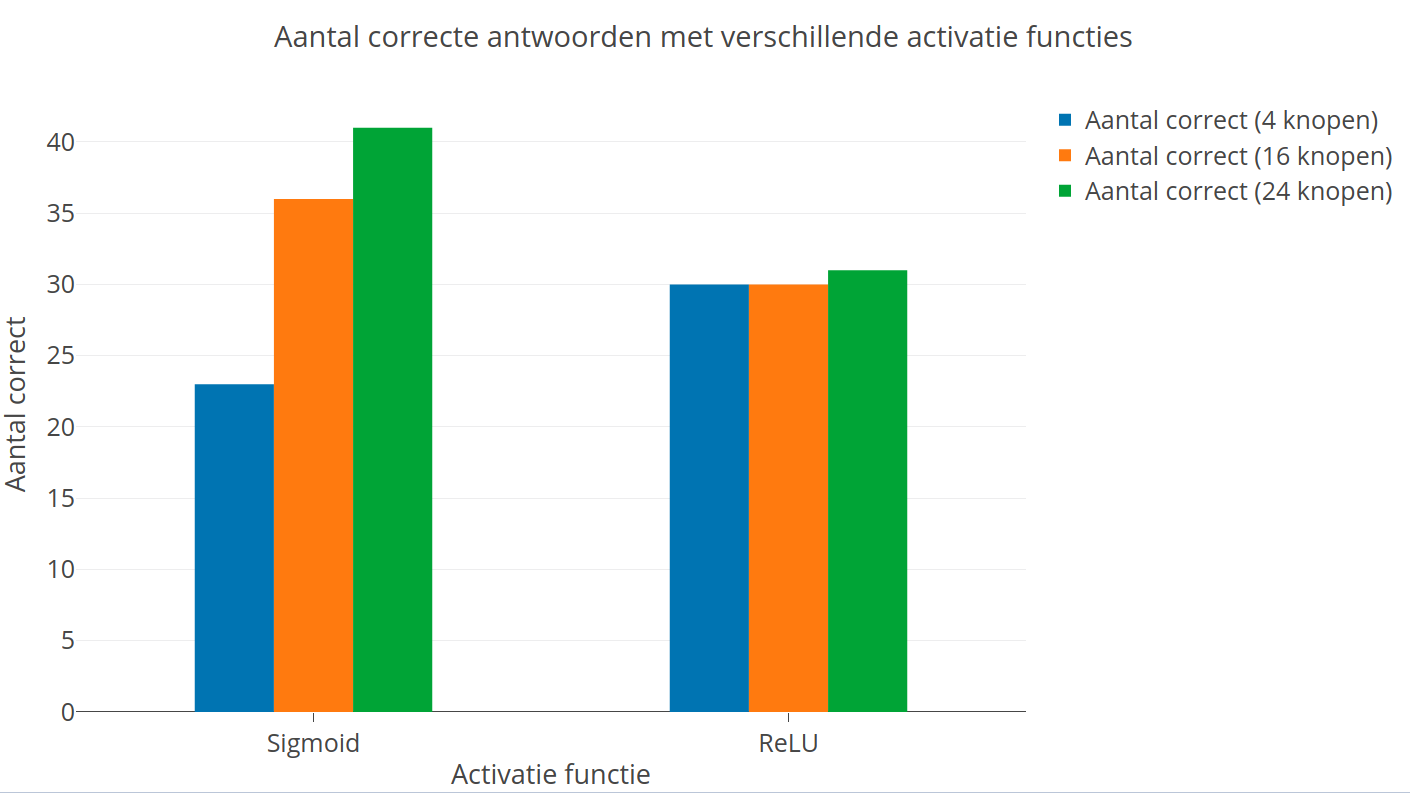
\includegraphics[scale=0.3]{graphs/g.png}
    \caption{Grafiek van Tabel \ref{tab:relu}}
    \label{fig:relu}
\end{figure}

\clearpage
\begin{figure}[ht!]
    \centering
    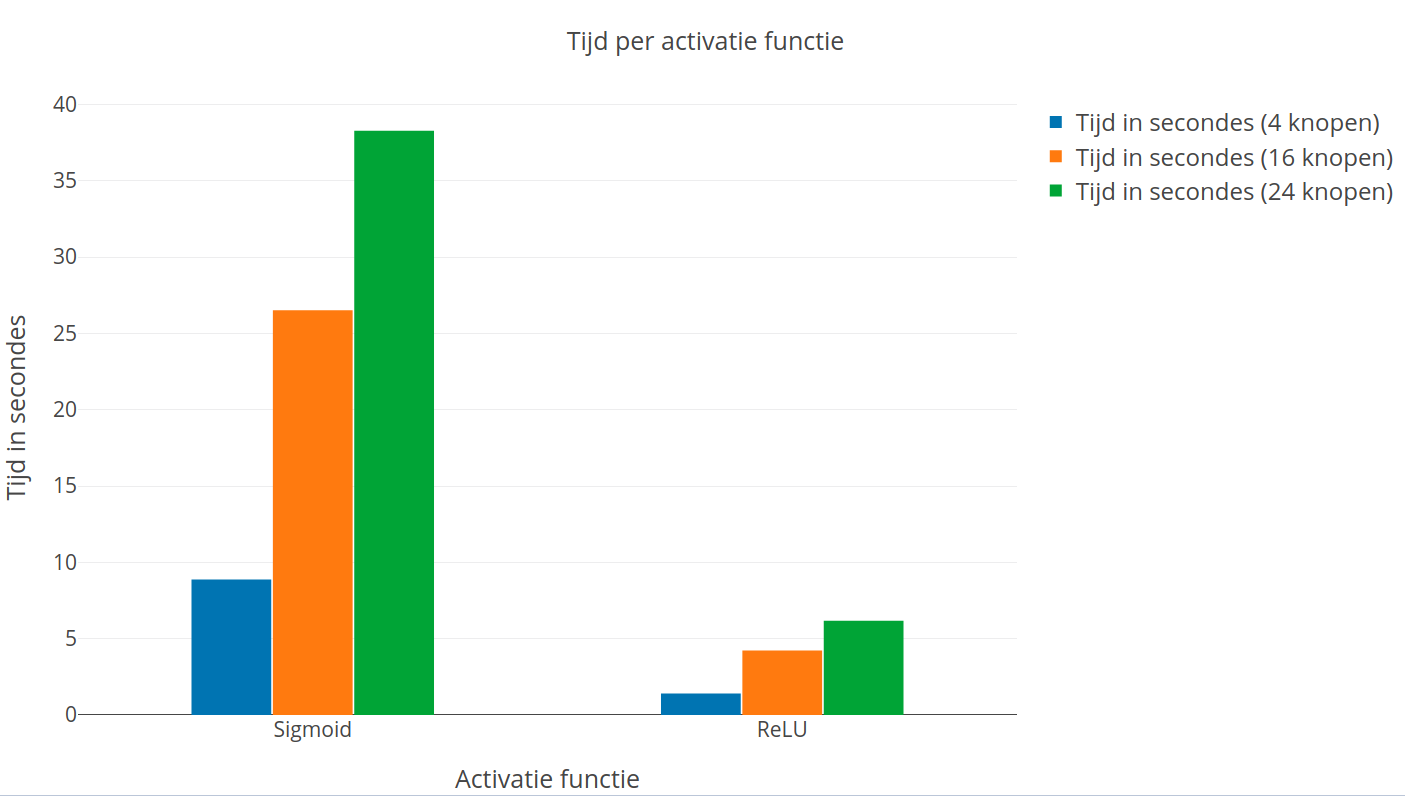
\includegraphics[scale=0.3]{graphs/time.png}
    \caption{Grafiek van de tijd in Tabel \ref{tab:relu}}
    \label{fig:relutime}
\end{figure}

\subsection{Keras netwerk}
Als laatste vergelijken we ons neuraal netwerk met een netwerk gemaakt met behulp van Keras \cite{keras}, een neuraal netwerk API. Het Keras netwerk is te vinden \href{http://liacs.leidenuniv.nl/~kosterswa/AI/samplekeras.tgz}{\underline{hier}} \cite{assignment}. 
Beiden netwerken zullen draaien met 10000 trainingssessies, 2 verborgen knopen met sigmoid als activatie functie en een leersnelheid van 0.01.

\begin{table}[ht]
    \centering
      $\begin{array}{l || c | c | c | c}
                                     & \text{Keras} & \text{Ons} \\ \hline
        \text{Percentage \% correct} & 51 & 0 \\ \hline
      \end{array}$
    \caption{Het Keras netwerk tegen ons neuraal netwerk}
    \label{tab:keras}
\end{table}